\section{Classification/Constraints of Elastic Moduli}
For a less detailed discussion of what we discuss here, you can consult chapter 9 (``Active Matter'') of the Soft Matter textbook.

\subsection{Summary of Last Lecture}
Last lecture, we studied solids, and the relationship between the stress and strain tensor:
\begin{equation}
    \sigma_{ij} = K_{ijkl}\underbrace{u_{kl}}_{\p_k u_l}
\end{equation}
the two are related via the stiffness tensor $K_{ijkl}$, which summarizes the identity of the solid.

If the forces are conservative, then the stress is the variation of an energy density:
\begin{equation}\label{eq:sigmavariation}
    \sigma_{ij} = \dpd{\e}{u_{ij}}
\end{equation}
And it follows that $K_{ijkl}$ is symmetric under exchange of pairs of indices:
\begin{equation}\label{eq:reciprocity}
    K_{ijkl} = K_{klij}
\end{equation}

But, say we want to consider a medium where the forces are not conservative. Then neither of Eq. \eqref{eq:sigmavariation}, \eqref{eq:reciprocity} have to hold. In this more general case, we can split $K_{ijkl}$ into an even and odd part:
\begin{equation}
    K_{ijkl} = K^e_{ijkl} + K^o_{ijkl}
\end{equation}
where even/odd means that the tensor acquires a $\pm$ sign under swap of pairs of indices. In a soft matter or elasticity course you have seen the first term - but the second term is novel, and comes up when we study open systems.

Since the forces are non-conservative, work is no longer a state function:
\begin{equation}
    W_{AB} \neq U_B - U_A
\end{equation}
\begin{center}
    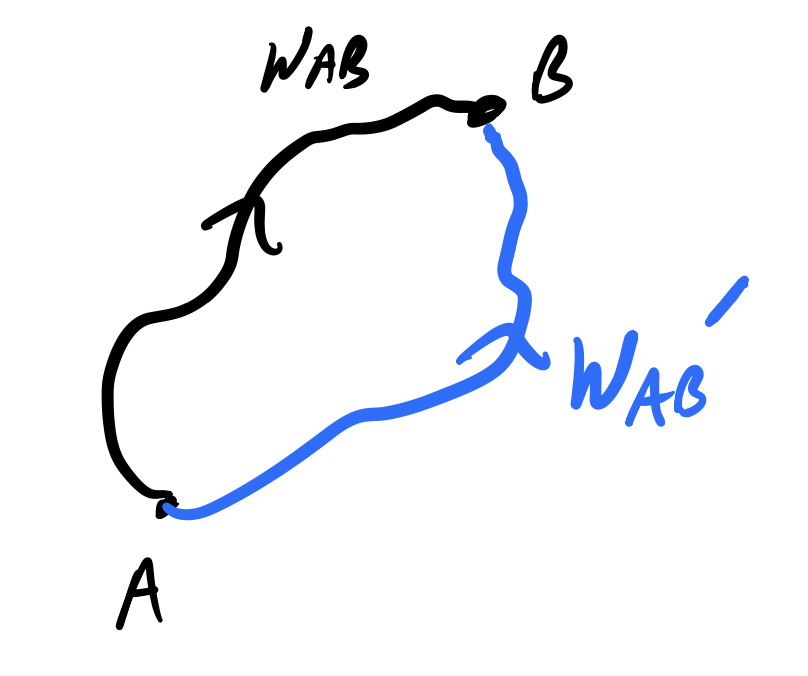
\includegraphics[scale=0.3]{Lectures/Images/lec2-work.png}
\end{center}
In this case, we have net work (positive or negative, depending on the sign) when we go around a cycle. The work done is rate-independent (no time derivatives here!). Further, the medium must be chiral because there is a difference in the sign of work depending on whether we traverse a loop clockwise or counterclockwise.

\subsection{Representations of Stress/Strain Tensors}
Let's try to classify all possibel entries of the stiffness tensor $K_{ijkl}$ using the representations of $\sigma$ and $u$; this will allow us to classify possible elastic moduli. In particular, let us try to classify odd elasticity $K^o_{ijkl}$ in 2-dimensions. In 2-D, stress $\sigma_{ij}$ and strain $u_{kl}$ each have 4-independent components, which we may package into a 4-entry vector. Therein the stiffness $K_{\alpha\beta}$ is a 4x4 matrix that connects them. We ``play God'' by analyzing/studying the form of $K_{\alpha\beta}$ without knowing any details about our system - we can deduce constraints purely mathematically.

\begin{center}
    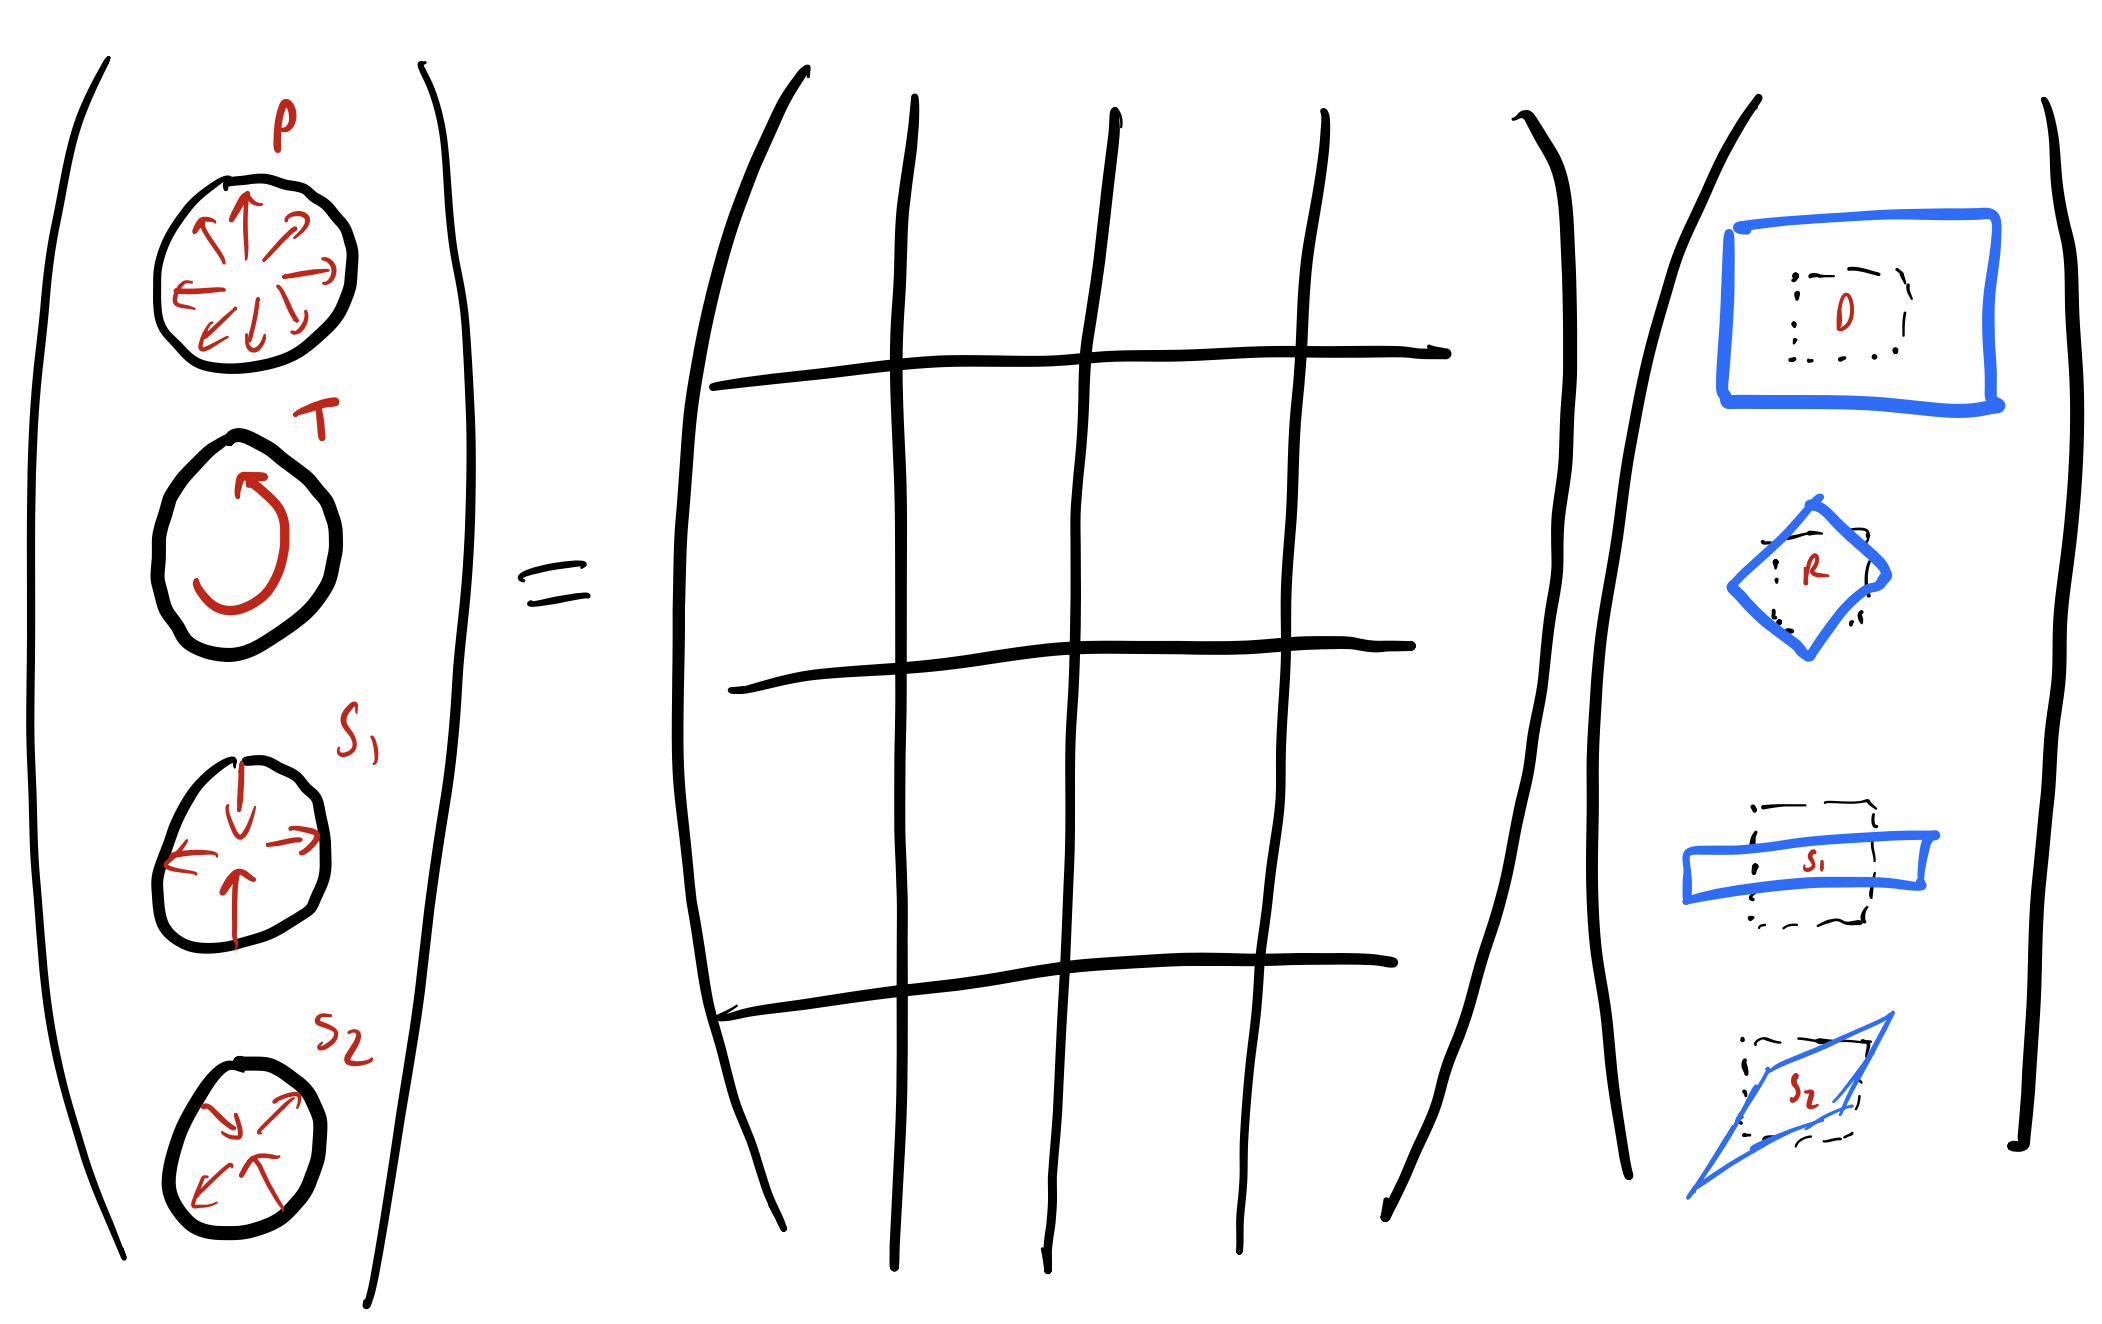
\includegraphics[scale=0.35]{Lectures/Images/lec2-stiffnessmatrix.png}
\end{center}
\begin{equation}
    \m{\text{P} \\ \text{T} \\ \text{SS1} \\ \text{SS2}} = \m{\cdot & \cdot & \cdot & \cdot \\ \cdot & \cdot & \cdot & \cdot \\ \cdot & \cdot & \cdot & \cdot \\ \cdot & \cdot & \cdot & \cdot}\m{\text{D} \\ \text{R} \\ \text{S1} \\ \text{S2}}
\end{equation}

The four entries of strain $u_{\beta}$ will be the projections onto the basis elements of dilation, rotation, 2 shears. We can do the same for stress, writing down the forces that result from the deformations - pressure, torque, and shear stress 1/2. Then the matrix elements of $K_{\alpha\beta}$ relate the two.

What is the analytical meaning of the drawings above? We write:
\begin{equation}
    u_{ij} = \sum_{\alpha=0}^3 u^\alpha \tau_{ij}^\alpha
\end{equation}
with:
\begin{equation}
    \tau^0 = \m{1 & 0 \\ 0 & 1}, \quad \tau^1 = \m{0 & 1 \\ -1 & 0}, \quad \tau^2 = \m{1 & 0 \\ 0 & -1}, \quad \tau^3 = \m{0 & 1 \\ 1 & 0}
\end{equation}
Corresponding to dilation, rotation, shear 1, and shear 2 respectively. Note that these obey the relation (note that we take a trace below, since the indices are repeated and hence summed):
\begin{equation}
    \boxed{\tau_{ij}^\alpha \tau_{ij}^\gamma = 2\delta^{\alpha\gamma}}
\end{equation}
This is the algebra for the generators of the rotation group in 2-D.

This was a statement about the geometry of the strain deformation. We can do a similar procedure for the stress:
\begin{equation}
    \sigma_{ij} = \sum_{\alpha=0}^3 \sigma^\alpha \tau^\alpha_{ij}
\end{equation}
where now the projections onto $\tau^0, \tau^1, \tau^2, \tau^3$  correspond to pressure, torque, shear stress 1, shear stress 2.

\subsection{Classifying elastic moduli}
Now, we want to discover what is in the $K_{\alpha\beta}$ matrix. To this end, we can think about symmetries of the medium. One such symmetry/idea is isotropy - wherein there is no preferred direction to the material. With this assumption we can already set a lot of the entries of $K$ to zero. 

In a world that is isotropic, I cannot couple a scalar/pseudoscalars to a vector/bivectrs - why? Because this would involve a preferred direction. So, look at the matrix element of $K$ that connects dilation with shear stress. We cannot measure the angle of shear in a isotropic medium, so this matrix element must vanish.

More generally, the dilation/rotation subspaces are scalar/pseudoscalars, and the stress subspaces are pseudovectors. Further, pressure/torque are scalar/pseudoscale and shear stress are pseudovector. By isotropy the subspaces cannot be connected, which allows us to conclude that 8 of the entries vanish:

\begin{equation}
    \m{\text{P} \\ \text{T} \\ \text{SS1} \\ \text{SS2}} = \m{\cdot & \cdot & 0 & 0 \\ \cdot & \cdot & 0 & 0 \\ 0 & 0 & \cdot & \cdot \\ 0 & 0 & \cdot & \cdot}\m{\text{D} \\ \text{R} \\ \text{S1} \\ \text{S2}}
\end{equation}

Next, consider the symmetry of objectivity/frame invariance. We can consider the solid to be ``self-standing'' - in this case, applying a rigid body rotation applies no stress. Note that we can break this if the solid was standing on some sticky surface (in which case we could have stresses applied from the contact) - symmetries can be broken by perturbations, e.g. isotropy via a magnetic field. But what does this frame invariance give us for the stiffness tensor? Since rotation generates no stresses, the entire second column is set to zero (rotations cannot generate pressure or torques).

\begin{equation}
    \m{\text{P} \\ \text{T} \\ \text{SS1} \\ \text{SS2}} = \m{\cdot & 0 & 0 & 0 \\ \cdot & 0 & 0 & 0 \\ 0 & 0 & \cdot & \cdot \\ 0 & 0 & \cdot & \cdot}\m{\text{D} \\ \text{R} \\ \text{S1} \\ \text{S2}}
\end{equation}

We have assumed that linear momentum is conserved. We have not used energy conservation here - let's see what this implies for us now.

To learn about the last remaining entries, let us work through some algebra. We write:
\begin{equation}
    \sigma_{ij} = \textcolor{blue}{\sigma^\gamma \tau^\gamma_{ij}} = K_{ijkl} = u_{kl} = \textcolor{blue}{K_{ijkl}\tau^\beta_{kl}u^\beta}
\end{equation}
Now multiplying the blue by $\frac{1}{2}\tau^\alpha_{ij}$, then on the LHS I get:
\begin{equation}
    \frac{1}{2}\tau^\alpha_{ij}\sigma^\gamma \tau^\gamma_{ij} = \frac{1}{2}\sigma^\gamma 2\delta^{\alpha\gamma} = \sigma^\alpha
\end{equation}
and on the RHS we get:
\begin{equation}
    \frac{1}{2}\tau^\alpha_{ij} K_{ijkl}\tau^\beta_{kl}u^\beta
\end{equation}
so:
\begin{equation}
    \sigma^\alpha = \frac{1}{2}\tau^\alpha_{ij} K_{ijkl}\tau^\beta_{kl}u^\beta = K^{\alpha\beta}u^\beta
\end{equation}
So, if we assume that the theory is conservative/we have reciprocity $K_{ijkl} = K_{klij}$, then $K^{\alpha\beta} = K^{\beta\alpha}$ - the matrix is symmetric, and so we can set the matrix element that connects dilation to torque is zero:
\begin{equation}
    \m{\text{P} \\ \text{T} \\ \text{SS1} \\ \text{SS2}} = \m{\cdot & 0 & 0 & 0 \\ 0 & 0 & 0 & 0 \\ 0 & 0 & \cdot & \cdot \\ 0 & 0 & \cdot & \cdot}\m{\text{D} \\ \text{R} \\ \text{S1} \\ \text{S2}}
\end{equation}
We can name some of the remaining entries; the entry connecting dilation to pressure is the bulk modulus $B$:
\begin{equation}
    \m{\text{P} \\ \text{T} \\ \text{SS1} \\ \text{SS2}} = \m{B & 0 & 0 & 0 \\ 0 & 0 & 0 & 0 \\ 0 & 0 & \cdot & \cdot \\ 0 & 0 & \cdot & \cdot}\m{\text{D} \\ \text{R} \\ \text{S1} \\ \text{S2}}
\end{equation}
Now, it is an exercise that you may have on a problem set that isotropy constrains the lower diagonal entries to be the same, and the lower off-diagonal entries to be equal and opposite. The diagonals we can call the shear modulus $G$, and the off-diagonals must be zero (as energy conservation constrains $K^{\alpha\beta}$ to be symmetric). Thus:
\begin{equation}
    \m{\text{P} \\ \text{T} \\ \text{SS1} \\ \text{SS2}} = \m{B & 0 & 0 & 0 \\ 0 & 0 & 0 & 0 \\ 0 & 0 & G & 0 \\ 0 & 0 & 0 & G}\m{\text{D} \\ \text{R} \\ \text{S1} \\ \text{S2}}
\end{equation}

So, if we assume isotropy, frame invariance, and conservative forces, we just have $B, G$ above. Let's repeat the analysis if we do not assume conservative forces. The diagonal components are not affected, but the off-diagonal entries we constrained to be zero are now generically nonzero:
\begin{equation}
    \m{\text{P} \\ \text{T} \\ \text{SS1} \\ \text{SS2}} = \m{B & 0 & 0 & 0 \\ A & 0 & 0 & 0 \\ 0 & 0 & G & -K^0 \\ 0 & 0 & +K^0 & G}\m{\text{D} \\ \text{R} \\ \text{S1} \\ \text{S2}}
\end{equation}

So, this is the conclusion of our analysis - we have (relaxing energy conservation) 4 moduli describing our material. 

Comment: In an anisotropic medium, we could have the moduli coupling the two shears, but they will \emph{not} be equal and opposite. One could then imagine matrix elements of the form $\e + K^0, \e - K^0$; one must look at the \emph{difference} to conclude nonconservative forces (just looking at one element, you cannot be sure if the source is anisotropy). Additionally, a nonzero $A$ does not necessarily mean nonconservative forces, it means nonconservative forces \emph{and} frame invariance, so to conclude nonconservative forces concretely we would need to compare with the other matrix element across the diagonal.

\subsection{Quantifying Work}
We derive the expression for the work coming from the stresses. For a force we have the contour integral:
\begin{equation}
    W = -\oint \v{F} \cdot d\v{l}
\end{equation}
For stresses, we consider a loop integral in 4-D space:
\begin{equation}
    W = -\oint \sigma_{ij}du_{ij} = -\oint \sigma^\beta du^\beta
\end{equation}
Now using Stokes' theorem:
\begin{equation}
    W = \iint \e^{\alpha\beta}\frac{\partial \sigma^\beta}{\partial u^\alpha}dA
\end{equation}
With $\e^{\alpha\beta} = \m{0 & -1 \\ 1 & 0}$. Now, we can use that $\sigma^\beta = K^{\beta\alpha}u^\alpha$, and take the derivative. Note that we can focus solely on the entries of the tensor coming from the non-conservative forces (the parts coming from conservative forces give trivially zero contribution)! Writing $K^{\alpha\beta} = K^0e^{\alpha\beta}$ (we focus on the subspace of shears), we get:
\begin{equation}
    W = -\iint \e^{\alpha\beta}e^{\beta\alpha}K^0 dA
\end{equation}
Then:
\begin{equation}
    \e^2 = \m{-1 & 0 \\ 0 & -1} \implies -\e^{\alpha\beta}e^{\beta\alpha} = 2
\end{equation}
and so:
\begin{equation}
    W = 2K^0 \cdot \text{Area}
\end{equation}
So we see that we do indeed have a nonzero amount of work, proportional to the odd elastic modulus and enclosed area.